\documentclass{TDP003mall}
\usepackage{titlesec}
\usepackage{graphicx}
\definecolor{terminalgreen}{HTML}{8AE234}

\newcommand{\version}{Version 0.1}
\author{Eric Jönsson, \url{erijo137@student.liu.se}\\
  Ida Bergquist, \url{idabe112@student.liu.se}}
\title{Systemdokumentation}
\date{2018-10-16}
\rhead{Ida Bergquist\\
Eric Jönsson}



\begin{document}
\projectpage
\tableofcontents
\newpage
\section{Revisionshistorik}
\begin{table}[!h]
\begin{tabularx}{\linewidth}{|l|X|l|}
\hline
\textbf{Ver.} & \textbf{Revisionsbeskrivning} & \textbf{Datum} \\\hline
0.1 & Skapade systemdokumentationen & 181016 \\\hline
\end{tabularx}
\end{table}

\section{Overview}
\begin{figure}[h!]
    \centering
    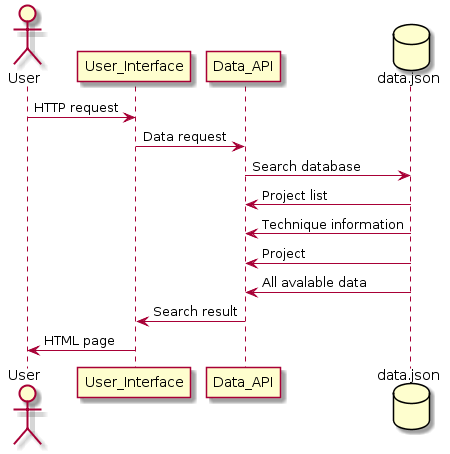
\includegraphics[width=10cm]{sevenskdiagram.png}
    \caption{Simplified view of the portfolio}
    \label{sekvensdiagram}
\end{figure}

\section{Design}
\subsection{Data API}
All functions are defined in a seperate document called module documentation.
\subsection{User interface}
\begin{figure}[h!]
    \centering
    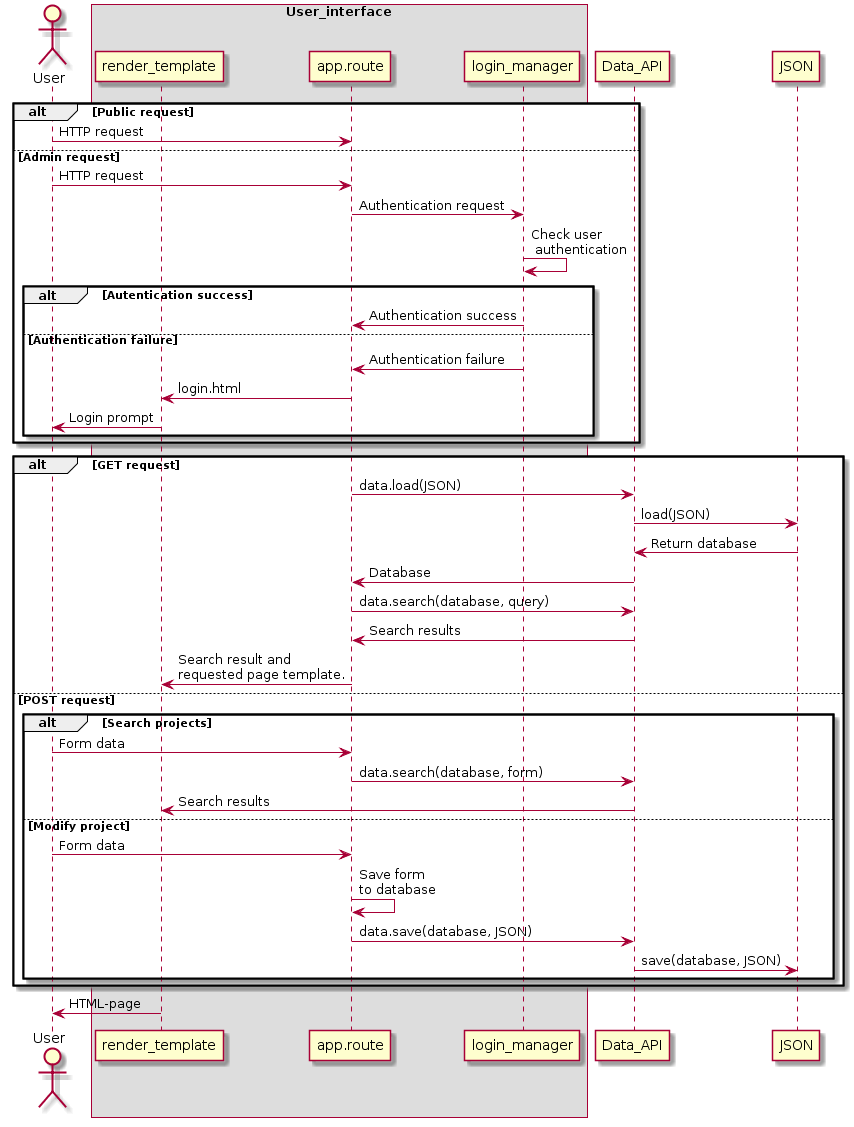
\includegraphics[width=\linewidth]{sekvensdiagram2-3.png}
    \caption{The inner workings of the user interface}
    \label{sekvensdiagram2}
\end{figure}
All functions
\section{Errors and errorlogs}


\end{document}
